\documentclass[12pt]{article}
\usepackage{palatino} %  Sets typeface as Palatino
%\usepackage{times}    %  Sets typeface as Times
%\usepackage{newcent}  %  Sets typeface as New Century Schoolbook
%\usepackage{bookman}  %  Sets typeface as Bookman
%
%\usepackage{pictex}   %  use to activate pictex
%\usepackage{eurosym}  %  use \euro to make a Euro symbol
\usepackage{fancyhdr,xspace}
\usepackage{graphicx,epstopdf}  % Use for graphics with TeXShop
%\usepackage{geometry}
%\usepackage{dcolumn}    % Controls number of decimal places in tabular
%\usepackage{steinmetz}  % phase and angle notation
%\usepackage[printonlyused,withpage]{acronym}
%\usepackage{color} %  color for soul, \rx-\cx for type color
%\usepackage{ulem}  %  underlining, etc
%\usepackage{soul}  %  underlining, etc  (needs color.sty)
\usepackage{lastpage,float}
\usepackage{draftwatermark}       % This puts DRAFT across each page
%
\usepackage{latexsym, amssymb}   % include for mathematical symbols
%
%\usepackage[textures]{changebar} % use \cbstart and \cbend around changes
%\usepackage[pdftex]{changebar}   % \cbdelete creates a fat change bar
%
%\usepackage[xcolor=pdftex]{changes}      % text change mark-up utility
%\definechangesauthor{EW}{orange}         % EW changes in orange
%
\pagestyle{fancy}
%
\lfoot{\scriptsize{AVNA-Documentation.tex}}  % Put File Name Here}}
\cfoot{\thepage\ of \pageref{LastPage}}
\rfoot{\scriptsize{\today}}
\lhead{}
\chead{}
\rhead{AVNA Documentation V0.83}
%
\title{\textbf{AVNA User's Manual}}
\author{Bob Larkin W7PUA \\ Evans Wetmore K3VFA} %  name \\ address \\ and so on
%
\newcommand{\q}[1]{\textquotedblleft#1\textquotedblright} % puts text in quotes
\newcommand{\horizl}[1]{\makebox[#1]{\hrulefill}} % horizontal line
\newcommand{\degr}[1]{#1\mbox{\raisebox{4pt}{$\circ$}\hspace{-.5pt}}\hspace{.5mm}}
\newcommand{\vecr}[1]{\raisebox{8pt}{$\rightharpoonup$}\hspace{-11pt}\textbf{#1}}
\newcommand{\eg}{\textit{e.g.}, }
\newcommand{\ie}{\textit{i.e.}, }
\newcommand{\moca}{\textsf{MOCA}\textsuperscript{\texttt{R}\hspace{-6.8pt}$\bigcirc$}\xspace}
\newcommand{\ebno}{$E_b/N_0$\xspace}
\newcommand{\sqft}{ft\textsuperscript{2}\xspace}
\newcommand{\sqin}{in\textsuperscript{2}\xspace}
\newcommand{\sqm}{m\textsuperscript{2}\xspace}
\newcommand{\uvm}{${\mu}V/m$\xspace} % microvolts per meter
%\newcommand{\rx}[1]{\textcolor{red}{#1}}     % red text [color.sty]
%\newcommand{\gx}[1]{\textcolor{green}{#1}}   % green text [color.sty]
%\newcommand{\bx}[1]{\textcolor{blue}{#1}}    % blue text [color.sty]
%\newcommand{\yx}[1]{\textcolor{yellow}{#1}}  % yellow text [color.sty]
%\newcommand{\mx}[1]{\textcolor{magenta}{#1}} % magenta text [color.sty]
%\newcommand{\cx}[1]{\textcolor{cyan}{#1}}    % cyan text [color.sty]
%
%\newcolumntype{d}[1]{D{.}{.}{#1}}   % for decimal columns [dcolumn.sty]
%                                      #1 is number of decimal places
%
%\renewcommand{\abstractname}{Executive Summary} % Changes "Abstract" to
%                                                   "Executive Summary"
%
%\renewcommand{\familydefault}{\sfdefault} % makes sans serif font default
%
%\renewcommand{\familydefault}{\ttdefault} % makes typewriter font default
%
%\renewcommand{\baselinestretch}{2} % Turns on double-spacing
%\normalsize                        % This is also needed for double spacing
%
%\SetWatermarkText{CONFIDENTIAL}   % This replaces DRAFT with CONFIDENTIAL
%\SetWatermarkScale{0.7}           % The {0.7} sizes CONFIDENTIAL
%
\begin{document}
\addtocounter{secnumdepth}{2} % This allows subsubsections to be numbered
\addtocounter{tocdepth}{2} % This allows subsubsections in Table of Contents
%
%\input epsf.def 		% Turns on EPSF Macro
%
%\input BoxedEPS         % Turns on Boxed EPS Macro
%\SetTexturesEPSFSpecial % needed for Boxed EPS Macro
%\HideDisplacementBoxes  % turns off bounding boxes for Boxed EPS Macro
%
%\input{seteps}  % This sets up .eps graphics
%
%\input{picmacs.tex}  % Cut-and-Paste Pictures Macro
%
%\input{table}   % This enables Wichura Table Macro
%q	
\maketitle
\thispagestyle{fancy}
%
\tableofcontents
\listoffigures
%\listoftables
%
\restylefloat{table}  % allows use of [H] for tables--put it here!
\restylefloat{figure} % allows use of [H] for figures--put it here!
%
%\sffamily  % Puts Abstract in San Serif font
%\abstract{\textit{Text goes here}}
%\rmfamily  % Restores Roman Font for Remainder of Document
%
\setlength{\parskip}{0.15in} % Puts 0.25" between paragraphs

\part{Features and Capabilities}
The capabilities of Version 0.82 are the following:
\begin{itemize}
\item Audio Impedance Measurement
\item Audio Vector Network Analyzer (Audio Transmission Measurements)
\item Audio Spectrum Analyzer covering up to 40kHz with graphical display
\item Vector Voltmeter with frequency selectivity and adjustable phase offset
\item Four Signal Generators (added together)  with calibrated output.
\item Weighted and Unweighted Noise Measurement
\item Envelope and Group Delay Measurement
\item Screen Save to BMP file for all functions
\item Calibration of input and output levels and for the touch screen
\item AVNA Control via Serial Port
\end{itemize}

\section{Power Up}When the AVNA is turned on, it starts with an "Audio Test Instrument" screen that allows selection of the function.  This is, as usual, selected by the six touch screen buttons at the bottom of the screen.  In addition, if an $\mu$SD card is present in the Teensy 3.6 socket, a button with "S"  shows in the upper right corner for "Screen Save".

\begin{figure}[H]
\begin{center}
\includegraphics[scale=0.75]{zAVNA_Home}
\caption{Power-up Screen}
\label{power-up-label}
\end{center}
\end{figure}

At startup, the Serial Monitor shows the status of the $\mu$SD card followed by a directory listing. For example: 
\begin{itemize}
  \item Initializing SD card...and a card is present.
  \item Partition found: FAT32
  \item Volume size (Mbytes): 7378
  \item Files found on the card (name, date, time, and size in bytes):
  \begin{itemize}
   \item AVNA1\_00.BMP  2000-01-01 01:00:00 230454
   \item AVNA1\_01.BMP  2000-01-01 01:00:00 230454
   \end{itemize}
\end{itemize}

\textbf{Note:} $\mu$SD cards have grown in GB capacity over the years.  There may be problems with large capacity cards greater than 8 DB..

\section{Audio Impedance Measurement}
\label{sect:ZMeas}
%
Audio Vector Network Analysis (AVNA) measurements break into two main types,  reflection and transmission.  This section covers the first case, reflection.  The major use of reflection measurements is to determine the impedance
which creates the reflection, or, put another way, a quantity directly associated with impedance, such as inductance. This section covers AVNA impedance measurements. The next section covers transmission measurements.

The term "Vector" refers to the fact that we always measure both the amplitude and the relative phase of impedance.  This enables us to measure a combination of resistive and reactive components.
%
\subsection{Description}
\label{subsect:ZDescr}
Before getting to the details of the measurements, we need to explore a few background items.

\subsection{Complex Impedance}Using the AVNA1 impedance (Z) terminals , the basic measurement quantity that is often displayed is impedance described by a resistance in series with a reactance. The reactance can be either a lossless inductance or a capacitance. Mathematically, this is represented as a complex number \vecr{Z}=R+jX where R is the series resistance and X is the series reactance, both in Ohms. The AVNA1 uses complex-arithmetic notation for \vecr{Z} which allows mathematically sound computation to be done on circuit models; the user can think of it as a way to keep the resistance separate from the reactance.

If the reactance is positive, the series component represents an inductor. Likewise, if the reactance is negative, the series component is a capacitor.  Note that this is only one of many representations. As an example, a series configuration can be converted to a parallel pair of components, neither being the same value as the series pair.  We will not attempt to cover all the possibilities here, but a few of them will be described below, as they appear in the display.

\subsection{Reference Resistance}Two different reference resistances can be used with the AVNA, 50 and 5,000 Ohms. The best value to use is generally the one that is in the range of the measured values. It is easy to pick 50 Ohms if the measured value is, say, 10 + j100. If the series reactance is much larger than the series resistance, we have a high-Q component that is not the easiest to measure with an AVNA. For that case we are probably going to uses the reference resistance that is closest to \(X\) since that determines the component value. If the user is trying to measure a resistance value, it is best to pick a reference resistance closest to the resistor value.

A more elaborate procedure for finding the best reference resistance for a general impedance type is to first measure with 50 Ohms. Then find the geometric mean of the resistance and the reactance, that is \(\sqrt{R X}\). Then remeasure with 5,000 Ohm reference. Choose the ratio of the geometric mean to the reference resistance (50 or 5,000) which is closest to 1.0.

Closest in all these decisions means by ratio, not by subtraction. For instance 4,000 Ohms has a ratio with 50 Ohms of  \( \frac{4000}{50} = 80\) whereas the ratio with 5,000 Ohms is \( \frac{5000}{4000} = 1.25\). The latter is closer to 1.0 than the former.  Note that we put the larger value on top of the ratio for convenience in comparing the two results.
%
\subsection{Instructions}
\label{subsect:ZInstr}
\textbf{Getting Started - }Here is a step-by-step description of a single frequency impedance measurement followed by a description of a swept impedance measurement. This will all be done directly from the touch screen. Everything covered here, and more, can be done via the USB-Serial link, as is described in the "AVNA1 Serial Control" section.

When the AVNA1 is powered up you have a choice of four Audio Test Instruments along with Service and Calibration functions.
\begin{figure}[H]
\begin{center}
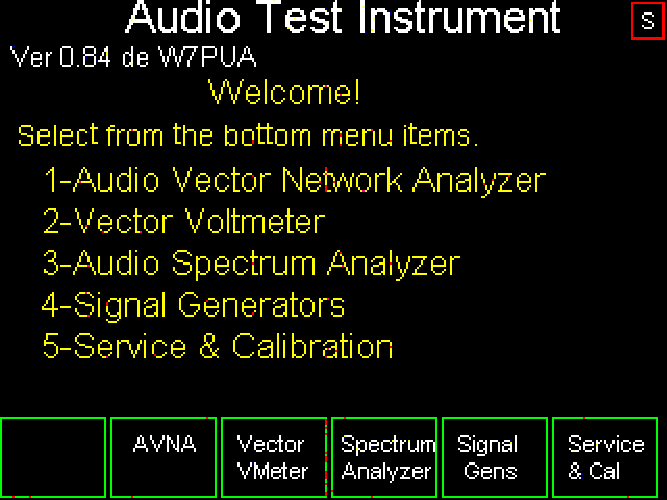
\includegraphics[scale=0.75]{./images/AVNA_000.pdf}
\caption{Audio Test Instrument Home  Screen.}
\label{AVNA_000-label}
\end{center}
\end{figure}
%
Referring to Figure \ref{AVNA_000-label}, we are now at the main AVNA1 Audio Test Instrument home screen.  For our impedance measurements, we will select the menu item, "\textsf{AVNA}" by touching that box at the bottom of the screen leading to the AVNA main screen.
\begin{figure}[H]
\begin{center}
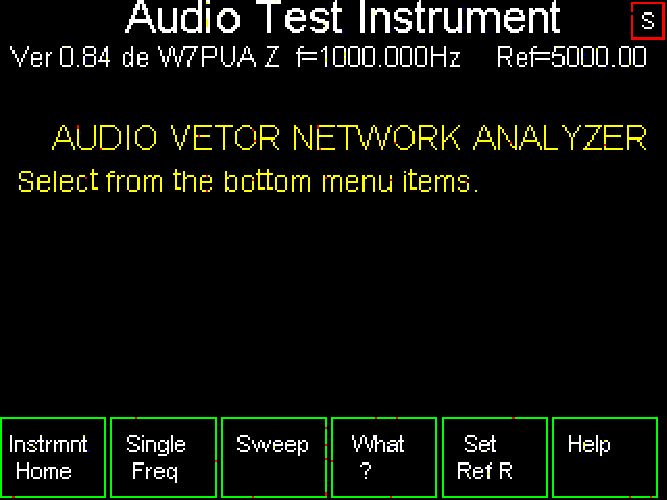
\includegraphics[scale=0.75]{./images/AVNA_001.pdf}
\caption{AVNA Main  Screen.}
\label{AVNA_001-label}
\end{center}
\end{figure}
%
We now have the choice  of single frequency or swept measurements as well as changing of the Reference Resistance described above. A last choice is the "What?" function for exploring components without knowing much about them. To continue our impedance measurement, we select "\textsf{Set Ref R}".
\begin{figure}[H]
\begin{center}
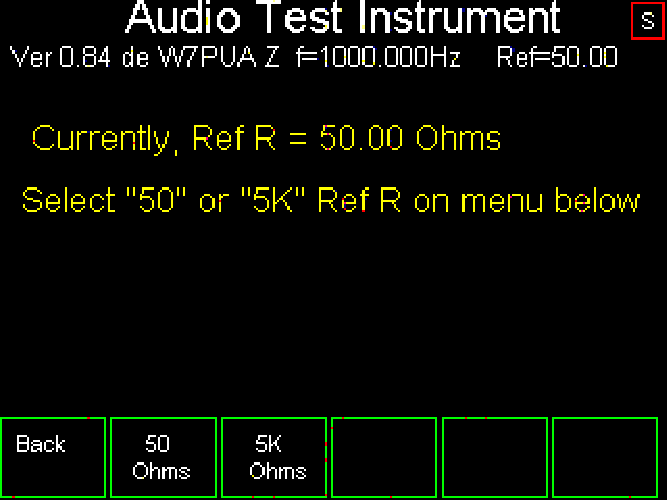
\includegraphics[scale=0.75]{./images/AVNA_003.pdf}
\caption{AVNA reference resistor selection  Screen.}
\label{AVNA_003-label}
\end{center}
\end{figure}
%
The current reference, as described above, is shown on the screen. It is also shown, during AVNA measurements, at the top of the screen in small type. Selecting the current value has no effect, and so we choose the menu item, "\textsf{5k Ohms}".
\begin{figure}[H]
\begin{center}
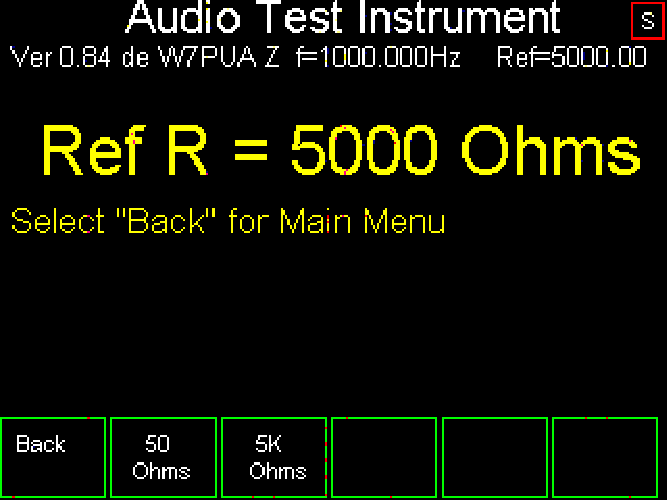
\includegraphics[scale=0.75]{./images/AVNA_004.pdf}
\caption{AVNA reference resistor selection of 5000 (5K) Ohms.}
\label{AVNA_004-label}
\end{center}
\end{figure}
At this point we have changed the reference resistance and can return to the AVNA main screen, Figure \ref{AVNA_001-label}, by tapping the menu item, "\textsf{Back}".

\textbf{Measuring an Impedance - }As an example, suppose we put together a series combination of a 10 Ohm resistor and a 0.22 $\mu$F capacitor and put this across the \q{Z} terminals. To get started, we can measure this at a single frequency by tapping on the menu item, "\textsf{Single Freq}". The frequency can be selected from a list of 13 ranging from 10 Hz to 40 kHz by using the menu items, "\textsf{Freq Down}" and "\textsf{Freq Up}".  For this sample measurement set the frequency to "1000 Hz".  Next, the menu item, "\textsf{Meas Z}" is tapped to start a continuing series of impedance measurement, as shown next.
\begin{figure}[H]
\begin{center}
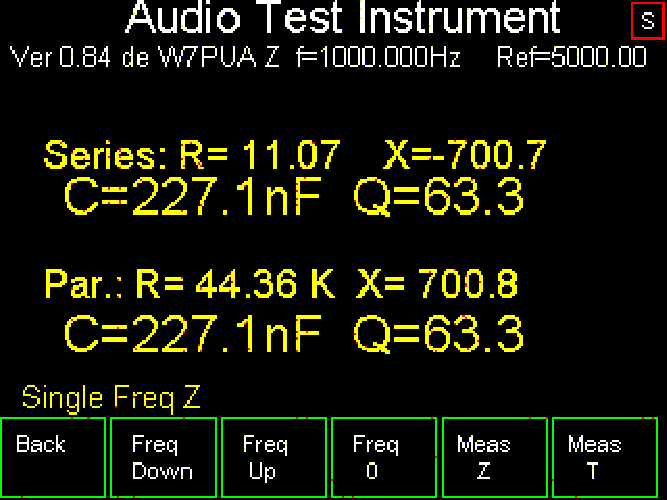
\includegraphics[scale=0.75]{./images/AVNA_006.pdf}
\caption{Impedance measurement of a series combination of 10 Ohms and a 0.22 $\mu$F capacitor.}
\label{AVNA_006-label}
\end{center}
\end{figure}
A couple of items to note:  First, this measurement repeats every second or so.
This is useful if you are measuring multiple components, or if you want to do mental averaging of the component values.

Next, we see the series combination of  \vecr{Z}=11.07 -j700.7, which is the resistance and reactance. I measured the 10 Ohm resistor, without the capacitor and saw 9.81 Ohms with a 50 Ohm reference and 8.23 Ohms with a 5000 Ohm reference, so the 11.07 Ohm value which is probably a combination of the difficulty in measuring the resistor with 700 Ohms reactance in series as well as some loss in the capacitor.  The 9.81 Ohms is very close to the measured DC value. Then we see the translation of the reactance value to a capacity of 227.1 nF (or 0.2271 $\mu$F).  Often this is the value we are looking for.

The Q value shown of 63.3 is the ratio of the reactance magnitude to the resistance value.  We are accustomed to measuring Q of inductors, and that would be shown here if the reactance was positive.  The Q of a capacitor has a physical meanings that parallels that of an inductor.

Lastly, the same screen shows the parallel RC values. At the one frequency where we measure the series connected components, we could have connected this parallel combination, and we would have measured the same quantities.
For more details on the series/parallel equivalence, see the original QEX article.\footnote{\textbf{\texttt{http://www.janbob.com/electron/AVNA1/Larkin-QEX-2018-May-Jun.pdf}}, pg. 12}
%
In particular, note that, in general, both the resistance and reactance values will change between the series and parallel representations.

\textbf{Swept Impedance Measurements - }  We do not have a graphical presentation of frequency swept impedance data.  Instead we have a tabular listing. To do this measurement from the single frequency version, we tap on "\textsf{Back}", bringing back the screen of Figure \ref{AVNA_001-label}. At this point we could change the reference resistor to 50 Ohms, but not for this exercise. Instead, we tap on "\textsf{Sweep}", bringing up the following screen.
\begin{figure}[H]
\begin{center}
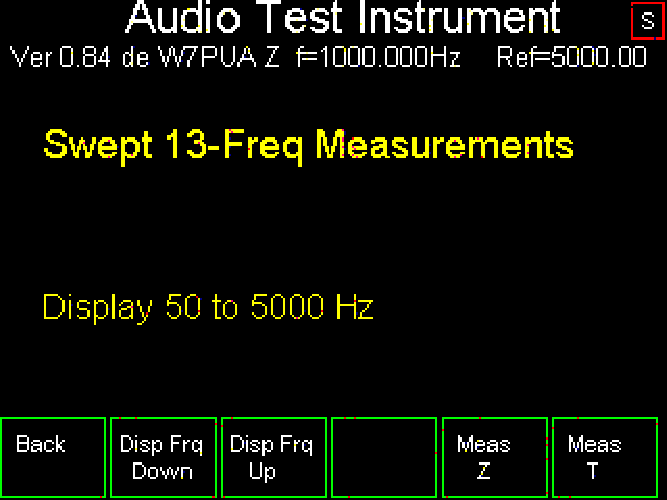
\includegraphics[scale=0.75]{./images/AVNA_007.pdf}
\caption{Main Screen for swept measurements.}
\label{AVNA_007-label}
\end{center}
\end{figure}
We can change the 7 screen displayed frequencies shown in Figure \ref{AVNA_009-label} with the two menu items at the bottom.  In all cases, the measurements are made at all 13 frequencies, but there is not room to display them all.  For now, we will leave the frequency settings at 50 to 5000 Hz.  We command the impedance measurement by tapping on, "\textsf{Meas Z}".  Here is the display.
\begin{figure}[H]
\begin{center}
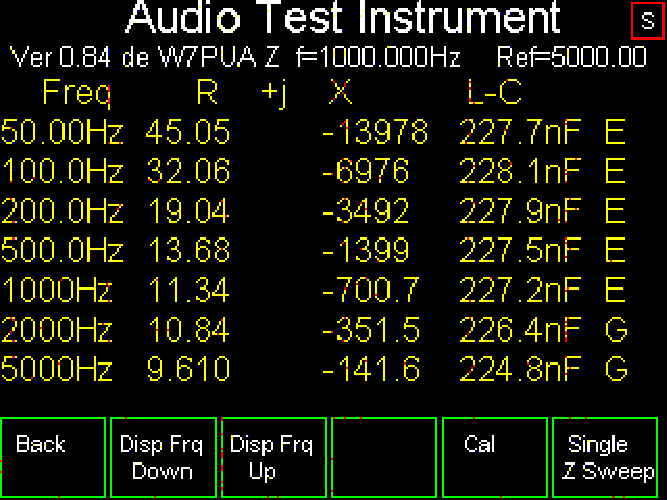
\includegraphics[scale=0.75]{./images/AVNA_009.pdf}
\caption{Swept impedance measurements.}
\label{AVNA_009-label}
\end{center}
\end{figure}
%
The display shows the impedance for seven frequencies.
The menu items, "\textsf{Disp Frq Down}" and "\textsf{Disp Frq Up}" allow the displayed frequencies to be shifted down or up to cover the entire 10 to 40,000 Hz range.  The impedance is shown in  \(R+jX\) format. It can be seen that negative reactance values display with a minus sign in front of the value. Next in the display line is a translation of the  \(jX\) value to either a capacitance or inductor value. The units, in this case,  "nF" change with component value.  In the right hand column is a rough measure of measurement quality. A single letter \textsf{E, G, P} corresponds to (\textsf{E})xcellent, (\textsf{G})ood, or (\textsf{P})oor. These indicate the difference between the impedance and the reference resistance.
The \textsf{E}, \textsf{G}, and \textsf{P} designations should not be taken too literally, but if the letter shows "\textsf{P}" or even "\textsf{G}",  you might consider the values and whether to re-measure with the other reference resistance.

Going back to the AVNA main menu, there is a menu item, "\textsf{What?}".  This is handy if the component type or value is unknown, or maybe a quick answer is wanted.  This starts with the following menu that describes what to do.
\begin{figure}[H]
\begin{center}
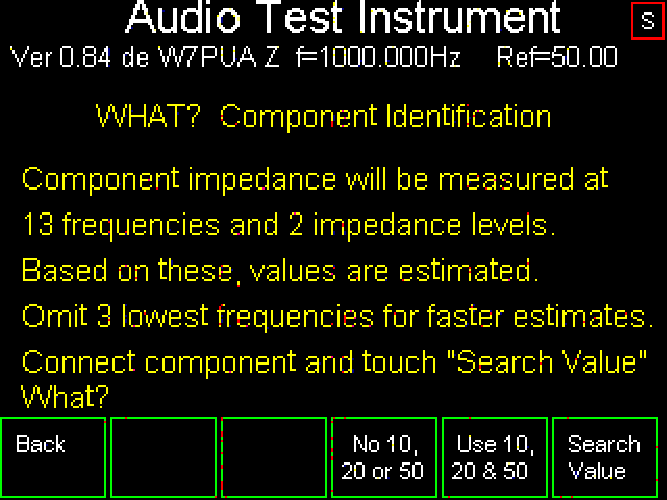
\includegraphics[scale=0.75]{./images/AVNA_012.pdf}
\caption{AVNA What? Screen.}
\label{AVNA_012-label}
\end{center}
\end{figure}
%
The only option available is to omit measuring at 10, 20 and 50 Hz that speeds up the measurement. Otherwise, tapping on "\textsf{Search Value}" produces the estimate:
\begin{figure}[H]
\begin{center}
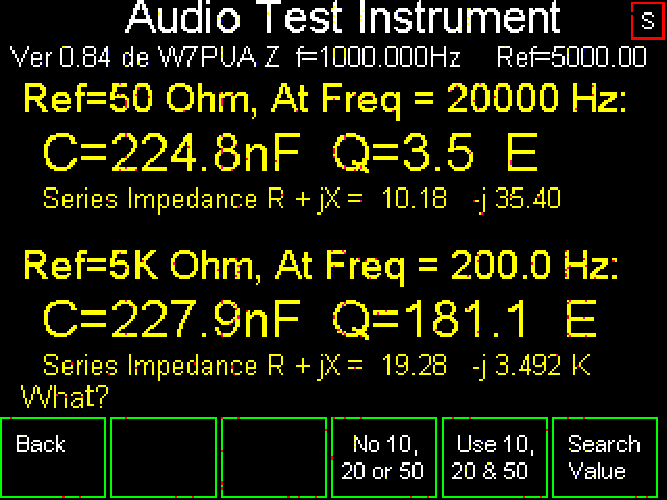
\includegraphics[scale=0.75]{./images/AVNA_013.pdf}
\caption{AVNA What? Screen after measuring.}
\label{AVNA_013-label}
\end{center}
\end{figure}
%
Two different values are shown, corresponding to the two reference resistor values.  The "\textsf{What?}" process chooses the frequency that gives an "E" for excellent measurement, if possible.  Often, this differs in frequency between the two reference resistor values.  For our 10 Ohm and 0.22 $\mu$F series combination, we find the 50 Ohm reference measurement at 20,000 Hz and the 5000 Ohm measurement down at 200 Hz.  In either case, the capacity value works out well, but measuring the 10 Ohm resistor in series with a 3492 Ohm reactance (at 200 Hz) is looking less successful with a 19.28 indicated \(R\) value.  It would be interesting to explore this further by measuring the two components individually with swept measurements. (We won't do that here to save the fun for others.)
%
\subsection{Discussion}
%
\textbf{Measurement Technique - } There are two commonly used methods of measuring impedance: the unbalanced Wheatstone bridge
%
\footnote{The classic Wheatstone bridge, \textbf{\texttt{https://en.wikipedia.org/wiki/Wheatstone\_bridge}}}
\footnote{The Wheatstone bridge in various AC/RF forms, \textbf{\texttt{http://g3ynh.info/zdocs/bridges/part\_1.html}}}
%
 and the series resistor method.   The latter method is used in the AVNA.
\begin{figure}[H]
\begin{center}
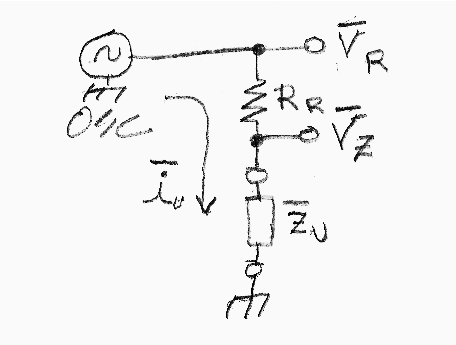
\includegraphics[scale=0.75]{./images/AVNA_900.pdf}
\caption{Functional schematic of impedance measuring circuit.}
\label{AVNA_900-label}
\end{center}
\end{figure}
%
Figure \ref{AVNA_900-label} shows the deceptively simple measurement circuit.  A software Direct Digital Synthesis (DDS) in the Teensy DSP creates a sine wave signal at a frequency between 10 and 40,000 Hz.  This is converted to an analog voltage by the left DAC on the Teensy Audio Adapter board which then goes to an audio amplifier producing the analog signal  \vecr{$V_R$} seen on the diagram.
The overhead bar indicates that this is a complex voltage where we care about the phase of the sine wave as well as the amplitude.  \vecr{$\mathbf{V_R}$} is applied to the series combination of our reference resistor, \(R_R\) and the unknown impedance, \vecr{$\mathbf{Z_u}$}.  This results in a current through the pair  of \(\vecr{$\mathbf{V_R}$}  /  (R_R +   \vecr{$\mathbf{Z_u}$})\) .  By measuring the complex voltage at the top of the unknown, \vecr{$\mathbf{v_Z}$} we can determine this current as
\begin{equation}
 \vecr{$\mathbf{i_u}$}=(\vecr{$\mathbf{V_R}$}-\vecr{$\mathbf{V_Z}$})/R_R
\end{equation}
 This in turn allows calculating the unknown impedance as
\begin{equation}
\vecr{$\mathbf{Z_u}$} =\vecr{$\mathbf{V_Z}$}/\vecr{$\mathbf{i_u}$}
                    =R_R\vecr{$\mathbf{V_Z}$}/(\vecr{$\mathbf{V_R}$}-\vecr{$\mathbf{V_Z}$})
\end{equation}
As one would expect, this requires knowledge of the reference resistor value, but the absolute voltages are not used, but rather the ratio of absolute voltages.  This makes it important to have the two voltmeters,\( \vecr{$\mathbf{V_R}$}\) and \( \vecr{$\mathbf{V_Z}$}\) track in both amplitude and phase.  There is separate analog circuitry in the two voltmeter paths, so errors will occur.  These errors are removed by the calibration procedure where the two voltmeters are connected to the signal source and the ratio  of voltages and the difference in phase of the two is recorded. These are then applied as corrections at each impedance measurement.

\textbf{Measuring Amplitude and Phase - }The discussion of Measuring Technique, above, refers to the two voltmeters that are needed.  The  implementation of voltmeters is discussed in the QEX article referenced above, pages 8-9,
and won't be repeated here.  The basic process is to generate a pair of software sine waves that are 90 degrees apart in phase but at the exact measurement frequency.  Each of these is multiplied (mixed) with the signal being measured and then low-pass filtered.  This produces the two complex voltages, needed for the impedance calculation.  All of the mixing and filtering occurs in the Teensy DSP.
\section{Audio Transmission Measurement}
This second major category of VNA measurements consists of generating a sine wave and applying this to some form of network.
 The network must have at least two sets of connections that act as the input and output.
The transmission measurement measures the input and output voltages and finds the ratio of the voltage magnitudes along with the difference in phase.
%
\subsection{Description}
\textbf{Complex Transmission - }The concept of voltage gain  is common.  
This is directly applied here when we take the ratio of the magnitude of the outpurt voltage to that of the input voltage.  
That measure does not involve the phase of the signals and is the same as applying a portable DVM to the terminals and dividing the result with a calculator.   
The "complex" or "vector" part comes in with phase measurement.  
Wth our VNA, we determine how much phase difference there is with the input and output sine waves.
This can be important for equipment such as  filters, control systems or communications networks.
It also is part of allowings a complete mathematical model of linear circuits to be constructed .  This can be a valuable tool for design of circuits.

It is worth noting that some of the concepts such as scattering parameters and reflection coefficients are applicable at low frequencies though they may be mainly thought of as RF descriptors.  Complex transmission (and impedance) measurements support these descriptors.  We won't attempt to cover all the possibilities here, but it would be an interesting topic for someone to explore.

\textbf{Measurement Transmission - }

\subsection{Instructions}
\textbf{Getting Started - }This procedure parallels the impedance measurements of the previos section.  We will cover the essence of a transmission measurement using the touch screen.
Everything covered here, and more, can be done via the USB-Serial link, as is described in the "AVNA Serial Control" section.

When the AVNA is powered up you have a choice of four Audio Test Instruments along with Service and Calibration functions as was shown before in Figure \ref{AVNA_000-label}.

\begin{figure}[H]
\begin{center}
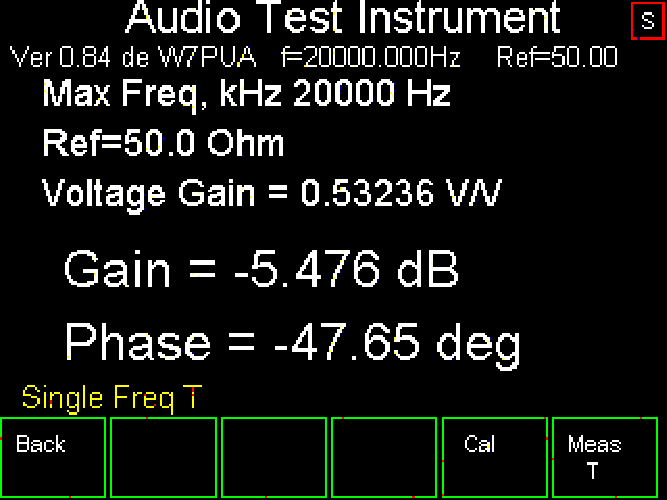
\includegraphics[scale=0.75]{./images/AVNA_029.pdf}
\caption{AVNA Transmission measurement for a single frequency.}
\label{AVNA_029-label}
\end{center}
\end{figure}
%
Referring to Figure \ref{AVNA_000-label}, we are now at the main Audio Test Instrument home screen.
We used to call this just, "the AVNA," but now we have added the other instruments like the Spectrum Analyzer, so this needs more descriptors.
For our impedance measurements, we will select the menu item, "AVNA" by touching that box at the bottom of the screen.
That  covers everything for the current discussion, leading to the AVNA main screen.

\begin{figure}[H]
\begin{center}
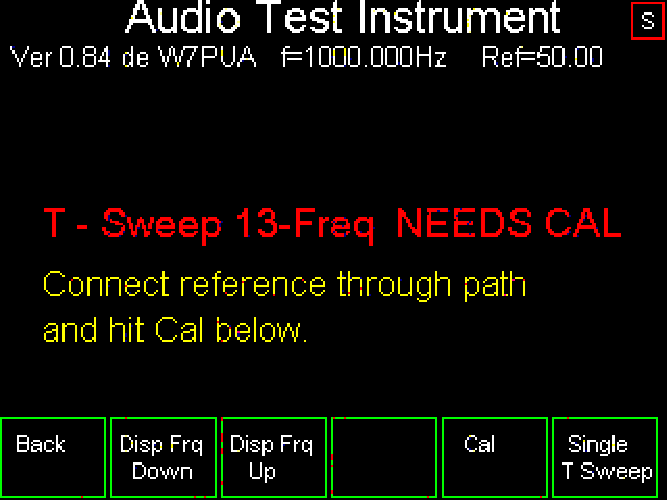
\includegraphics[scale=0.75]{./images/AVNA_031.pdf}
\caption{AVNA Transmission showing need for calibration.}
\label{AVNA_031-label}
\end{center}
\end{figure}
%

\begin{figure}[H]
\begin{center}
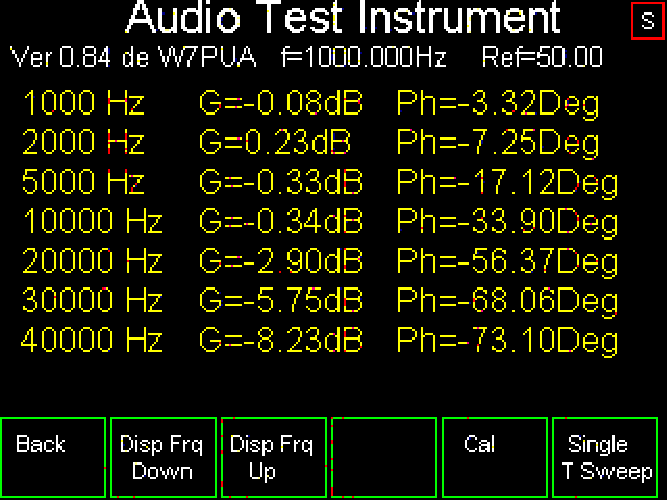
\includegraphics[scale=0.75]{./images/AVNA_032.pdf}
\caption{AVNA Swept Transmission measurement screen.}
\label{AVNA_032-label}
\end{center}
\end{figure}
%
\subsection{Discussion}
xxx

\section{AVNA Vector Voltmeter  (VVM)}
\label{sect:VVM}
The AVNA allows measurement of the gain of a device, using an internal signal generator.  This is presented in terms of dB change in amplitude and shift in phase angle between the input and output.  This most useful for characterizing a device, such as a filter.  To do this, we have indeed built a voltmeter to measure the device output.  But, sometimes we would just like to see the voltage displayed directly.  This lets us probe circuits for troubleshooting  and design work.   That is what the VVM does for us.

Phase information is important for some network diagnosis.  The VVM is intended to be used with the internal signal generator when phase is to be read.

\subsection{Description}
\label{subsect:VVMDescr}
The Vector Voltmeter measures the input rms voltage at any frequency up to about 40 kHz.  The frequency is set by the frequency of Signal Generator 1 (SG\#1).  Additionally, the phase difference between SG\#1 and the input signal is displayed.  By using the SG\#1 output to drive the test circuit, this phase is constant and can be a useful diagnostic tool.   If an external generator is used the measured phase difference will change at a rate determined by the frequency difference between the SG\#1 set frequency and the external generator.    This too can be a useful measurement.  

The bandwidth of the measurement is only a few Hz making it very sensitive, i.e., low noise.  The VVM operates down into the micro-volt  region.

\subsection{Instructions}
\label{subsect:VVMInstr}
\textbf{Using the VVM - }Operation starts  by setting the frequency of SG\#1 to that appropriate for the measurement.  The generator does not need to be enabled ("On") if the signal source for the measurement is generated externally.  If the internal SG\#1 is used as the signal source, it should be enabled and the amplitude set.   Only the frequency setting will affect the VVM measurement.  The steps for controlling the signal generator are listed in the Section 6, below.

If it is possible to do so, the internal SG\#1 should be used as the signal source, and this is a requirement if phase needs to be constant and representative of the circuit.

Again starting from the main home screen Figure \ref{AVNA_000-label}, we tap the "Vector VMeter" button on the bottom row.  This brings up the single screen used by the VVM.  It will be displaying amplitude in Volts, RMS  and phase in degrees, with both shown in bold numbers.  With no input, these should be low in value, with the exact voltage depending on frequency.  The example of Figure  \ref{AVNA_015-label} is running at 996 Hz, has the input shorted to ground, and shows 9 micro-volts RMS.
%
\begin{figure}[H]
\begin{center}
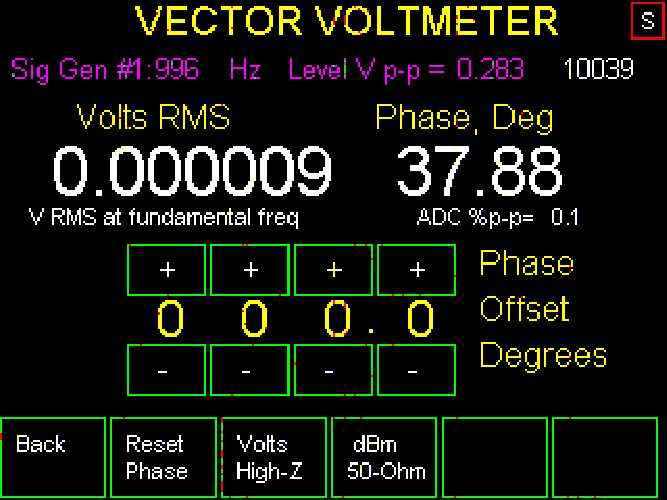
\includegraphics[scale=0.75]{./images/AVNA_015.pdf}
\caption{Vector Voltmeter, ready to measure but with no input.}
\label{AVNA_015-label}
\end{center}
\end{figure}
%
On the second from top text row is a notation, "SigGen \#1 996 Hz" that shows us the SG\#1 frequency without going back to the Signal Generator screens.  If SG\#1 is on (enabled) the frequency is shown in white, and otherwise it is shown in pink/red.

We can now measure a voltage at the chosen frequency by connecting an input to the T input terminals.  The voltage amplitude shown is valid regardless of whether the 50-Ohm switch is on or off.  The load of the 50-Ohms may cut the amplitude, but the voltage across the resistor is accurate.  Figure  \ref{AVNA_016-label} shows the resulting screen.
%
\begin{figure}[H]
\begin{center}
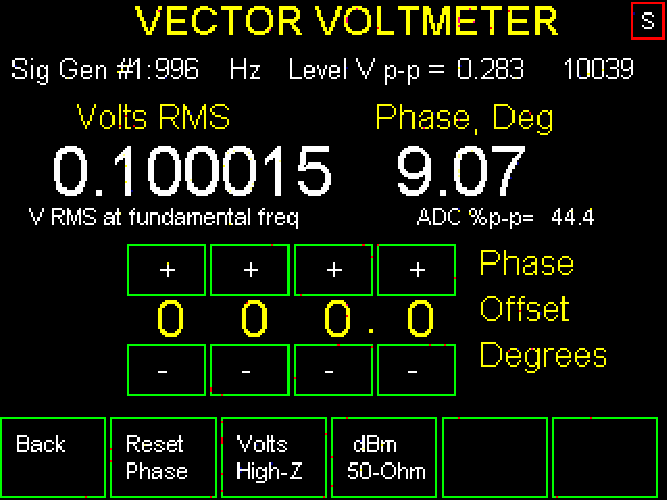
\includegraphics[scale=0.75]{./images/AVNA_016.pdf}
\caption{Vector Voltmeter with Sig Gen \#1 on and connected across to the VVM input.}
\label{AVNA_016-label}
\end{center}
\end{figure}
%
We can see that the input voltage is 0.100 Volts RMS..  From the second line, we see that the frequency of operation is 996 Hz, but it shows the level as 0.283 Vp-p.  These, of course, represent the same level  as the peak voltage is $\sqrt{2} = 1.414$ times the RMS voltage and peak-to-peak is twice the peak value.   This mixed units for the voltage is a complicated issue, probably makes sense but unfortunately causes more mental exercise than one might want, at times.

 Getting back to the VVM, you can see how close you are to overload by the little "ADC \%p-p=xx.x" on the screen.  This is the per cent of full ADC range for  the input.  If the level gets to 100\%, the voltage display turns red.  At that point the measurements are invalid.

Below the voltage and phase display is a "Phase Offset" input.  This can be set to values from -180 to +180 degrees.  This is a convenience that allows relative phase measurements to be made directly on the display.  This does not restrict the range of phase measurements, and they will always display between -180 and +180 degrees.

\textbf{Input Impedance - }One more convenience is the two buttons that select "Volts High-Z" or "dBm-50 Ohms."  For the  dBm readout to be correct, it is necessary to 50-Ohm terminate the input and that is easily done with the "50-Ohm" slide switch.  The resulting display  in Figure  \ref{AVNA_018-label} below.  Note that along with switching the amplitude units,  a phase offset that has been used to bring the phase display to 0.00 (almost).

When the 50-Ohm switch is not closed, the input impedance is1-Megohm in parallel with about 25 pF.  This is the input impedance of many oscilloscopes, meaning that  various x10 and x100 probes can be used with the VVM (as well as with the Spectrum Analyzer) to increase measurement voltage range and to ad isolation from a circuit being measured. \textbf{A Warning - }An oscilloscope comes with input protection circuits that we do not have with this box. That means that damage is easier to produce with the AVNA. Keep the input at the box to a Volt or so and everything will be OK. Big voltages can cause damage. 
%
\begin{figure}[H]
\begin{center}
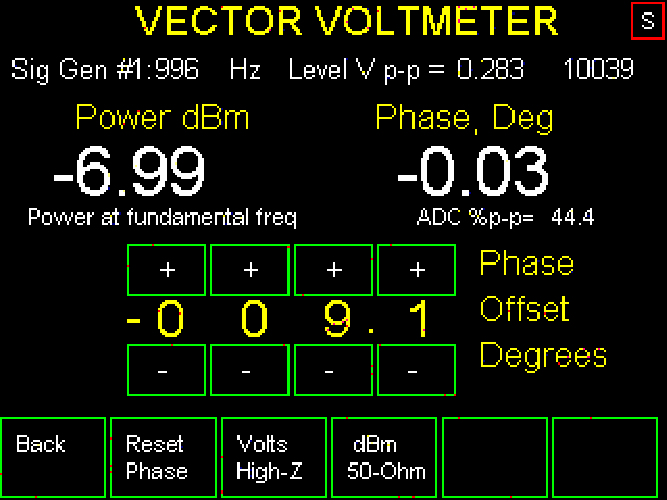
\includegraphics[scale=0.75]{./images/AVNA_018.pdf}
\caption{Vector Voltmeter with display set to power into 50-Ohms, expressed in dBm.}
\label{AVNA_018-label}
\end{center}
\end{figure}
%

One last note, if you are using an external signal source for VVM, and the measurements fails showing only microvolts, it is most likely that SG \#1 is not within a few Hz of the frequency of the input signal.  If the external source is not sufficiently stable, this may not be an appropriate method of measurement.  A broadband RMS voltmeter could be implemented, but that is for the future.

\subsection{Discussion}
\label{subsect:VVMDiscus}
The operation of the VVM is worthy of a few words. As a test instrument, it is closely related to the transmission measurements part of the Vector Network Analyzer AVNA). Much software is shared between the two instruments. The AVNA determines the relative gain or loss, amplitude and phase, through the transmission path. The VVM is calibrated so that the magnitude of the incoming signal is measured, along with the phase difference between Signal generator \#1 and that signal.

\textbf{DSP Circuit - }Two mixer (multiplier) outputs are the in-phase and quadrature signal levels. The square root of the sum of the squares of these two provides the magnitude of the incoming signal. The Signal Generator \#1 (SG \#1) sets the frequency of the measurement. Low pass filtering after the mixers sets the requirement that the incoming signal must be within a few Hz of the SG \#1 frequency. In many cases, it is easiest to just use the Signal Generator output on the Z terminals of the AVNA1 which is both on frequency and without having the phase changing with time.

If the SG \#1 signal is used as a signal source, the phase will not be shifting with time with time. For this the phase offset can be useful. This has up/down buttons to allow setting to 0.1 degree. The offset can be positive or negative. This sis a convenience for zeroing the displayed phase and does not change the basic measurement.

\textbf{Input Range - }The input needs to be within the range of the ADC. The maximum input is a little more than 0.2 Vrms or 0.6 V p-p.  Higher voltages require an external voltage divider.  The VVM can be used with the 50-Ohm input terminator, or not for which the input impedance is 1-megohm in parallel with around 25 pF.  In all cases, the VVM shows the voltage at the T input terminals.  The displayed voltage is the RMS value.  This is the same as HP used on the (now  old) 8405A VVM.   If the waveform is not sinusoidal, and there are harmonics, the displayed value is for the fundamental at the frequency of SG \#1.

The very narrow bandwidth of the VVM allows low level signals to be measured.  With SG \#1 turned off, I see a residual noise of about 10 micro-Volts.  But to use that, an external source generator is needed, with SG \# 1 tuned to the same frequency.  Otherwise, leakage through the CAL switch U4B in the AVNA causes a signal of about 55 uV with the 50 Ohm terminator or around 1.5 mV without.

\textbf{Single Channel Limitations - }The HP 8405 VVM has two inputs and phase-locked tuning to the reference input.  We only have one input channel, and so this feature cannot be supported.  But wait, there actually are two inputs.  If the AVNA was rewired to remove R46 to R49 and bring those leads to a switch and to a second input connector, a full 8405A style phase-locked loop could be implemented.  But, not now!


\section{Audio Spectrum Analyzer (ASA)}
\label{sect:ASA}
The AVNA project started with impedance and transmission analysis which is the normal set for a network analyzer.  However, the same hardware is capable of supporting other tests with the only changes being in the firmware.  This leads to a more general descriptor of "Audio Instrument."  One of the resulting instruments is the Spectrum Analyzer, covered here.  Note that, in addition to displaying spectra,  there some specialized tests for the measurement of Signal-to-Noise Ratio and SINAD.  These measurements are covered in this section as well, since they work as part of the Spectrum Analyzer.
\subsection{Description}
\label{subsect:ASADescr}
Within a frequency range of 10 Hz to 40 kHz, the power at the \q{T} input terminals is displayed.  Unlike instruments like the AVNA1, the display is graphical with power in dBm (relative to a milliwatt).  The frequency runs along the bottom axis and is always 0.0 at the left edge and up to 3, 6, 12, 24 or 48 kHz on the right side as chosen from the bottom-row menu.

The dBm calibration assumes an input resistance of 50-Ohms and that resistor should be switched in for the scale reference to be meaningful.  If the input does not have the 50-Ohms switched in, it has a 1-Megohm input impedance.  For the high impedance case, the 0 dBM line at the top corresponds to 0.223 V rms or 0.632-V p-p.

The dB per division and the dB offset for the dBm scale can be varied by the bottom-row menu.

As will be described in detail below, the spectrum analyzer can also do noise and  distortion measurements.

\subsection{Instructions}
\label{subsect:ASAInstr}
Everything starts with the Instrument Home screen shown in  Figure \ref{AVNA_000-label},  from which the user has a choice of four Audio Test Instruments. In this case we select, "\textsf{Spectrum Analyzer}"  which comes up sweeping with a 48 kHz width displaying an 80 dB range.   This is fine for many purposes and an input can be connected to the \q{T} input terminals.  Be careful to not input more than about 1-Volt p-p input or the ADC will be driven past its range, causing spurious response signals and inaccurate levels to be displayed.  Additionally, if the input level is very excessive,  damage can occur to the instrument.

\begin{figure}[H]
\begin{center}
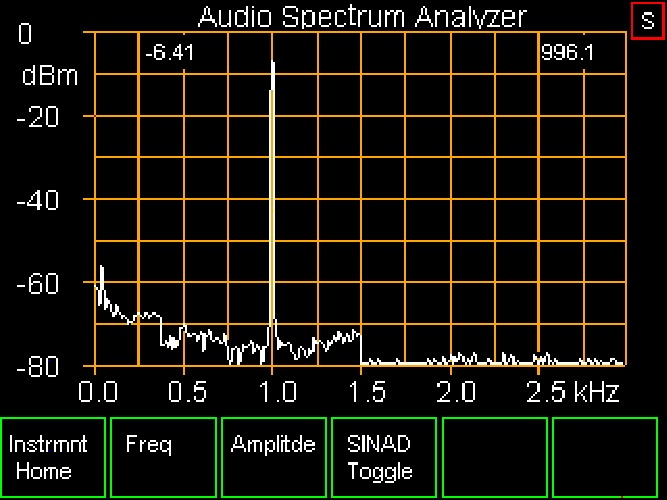
\includegraphics[scale=0.75]{./images/AVNA_019.pdf}
\caption{Spectrum Analyzer  showing a 996 Hz sine wave.  The frequency range has been reduced to 3 kHz by selecting a 6 kHz sampling rate. }
\label{AVNA_019-label}
\end{center}
\end{figure}
%
The screen should look somewhat like that in Figure \ref{AVNA_019-label}.  There will be no spike, as seen at about 1 kHz since there is no signal being applied and the frequency scale will default to 48 kHz.  The frequency scale will be different due to adjustments we will discuss in the next paragraph.  It is normal for the noise line to be higher on the left half of the screen and to rise to roughly -50 dBm at the very left edge.

\subsection{Frequency Coverage} To change the frequency range being displayed, we tap on the "\textsf{Freq}" button on the bottom row.  This brings up a screen allowing changes to the maximum frequency and describing the parameters  being used.  We have been talking about the maximum display frequency that has been set initially to 48 kHz.  The frequency changing control screen works in terms of "Sample Rate" that is twice the maximum display frequency being displayed.  In addition, a parameter, "\textsf{Maximum Frequency}" is shown that is 5/6 of the maximum display frequency.  This is unnecessarily confusing, but reflects that we can only work with inputs up to half of the ADC sampling frequency and further that there is a low-pass filter as part of the ADC that starts cutting off at about 5/6 of the half sampling frequency.  For the 96 kHz sampling frequency, this all means that the highest accurate measurement frequency is about 40KHz.  We show the full frequency range on the display, but we need to remember that the last two divisions on the screen are attenuated and should not be considered as numerically accurate.

So now we can change the total frequency range by adjusting the "\textsf{Sample Frequency}" down with the button on the bottom row.  The first button tap cuts the sample rate in half to 48 kHz.  If we continue tapping this button, we will get to the lowest range with a Sample Frequency of 6 kHz.  This will display 0 to 3 kHz as was seen in Figure  \ref{AVNA_019-label}.  We will later, under Signal Generators, see how to generate a sine wave as seen in the figure.


On the ASA frequency control screen,  we also see a numerical value for the Resolution Bandwidth.  This reflects the sampling rate as well as the 1024 point FFT being used.  In addition, resolution shown includes the 1.5 factor due to the Hann window function that is always used.\footnote{The resolution bandwidth of the FFT without windowing is the sampling rate divided by the number of sampling points per FFT, which in our case is 1024.  Windowing is used to reduce the spurious side signals due to taking a finite sample of the waveform.  See, \linebreak \textbf{\texttt{https://en.wikipedia.org/wiki/Window\_function}}}
%
Note that the FFT only gives 512 data points across the half-sample rate region.  There are 256 pixels available to display the data, so each pixel includes a little more than a single unit of FFT resolution.    The only setting involved with this is the Sample Rate setting and the remainder is automatic.

Finally, on the frequency screen there is provision for changing the amount of data averaging.  The advantage of averaging is to reduce the amount of noise seen on the spectral trace.  There are many times when this  increases the accuracy of measurements.  The penalty is slowness in the screen updates.

\subsection{Amplitude control} The vertical axis, when starting up, covers 80 dB of range with 10 dB per division.  The "\textsf{Amplitude}" button at the bottom of the Spectrum Analyzer screen brings up controls for dB per division (dB/div) and dB offset.  The db/div can be set to 20, 10, 5, or 2.  The offset comes in 5 dB increments and can be used to move the screen display up or down.  In all cases, the scale of dBm on the left axis tracks these changes.

\subsection{Marker annotation} Still looking at the Spectrum Analyzer screen, Figure  \ref{AVNA_019-label},  observe the "\textsf{-6.41}" notation at the top.  This is a measure, in dBm, of the amplitude of the strongest signal on the screen.  It assumes that the signal being measured is narrow band like the sine wave shown.  Over on the right side is a marking "\textsf{996.1}".  This is the estimated frequency of the same strongest signal using a clever method of interpolating the Hann windowed FFT.  \footnote{See, "A New Accurate FFT Interpolator for Frequency Estimation," \linebreak {\footnotesize\ \textbf{\texttt{ https://forum.pjrc.com/threads/36358-A-New-Accurate-FFT-Interpolator-for-Frequency-Estimation}}.}}
%
For reasonably strong signals, this estimated frequency is superior to conventional frequency counters. The estimate is being made in a fraction of a second, but accurate to around 0.1 Hz.   As you might expect, the accuracy diminishes at low signal-to-noise ratio, but still gives a useful estimate.

\subsection{SINAD and S/N} The last button on the main Spectrum Analyzer screen is a toggle that activates, or de-activates, some specialized measurements.  These use the same data as is displayed.  The measurement width is automatically set to 6 kHz (12 kHz sample rate) and the special measurements are made near 1 kHz.  There is no FFT bin centered on 1 kHz, so the nearest bin center of 996 Hz is really the center.  The display now looks like Figure \ref{AVNA_020-label}, but missing the signal.
%
\begin{figure}[H]
\begin{center}
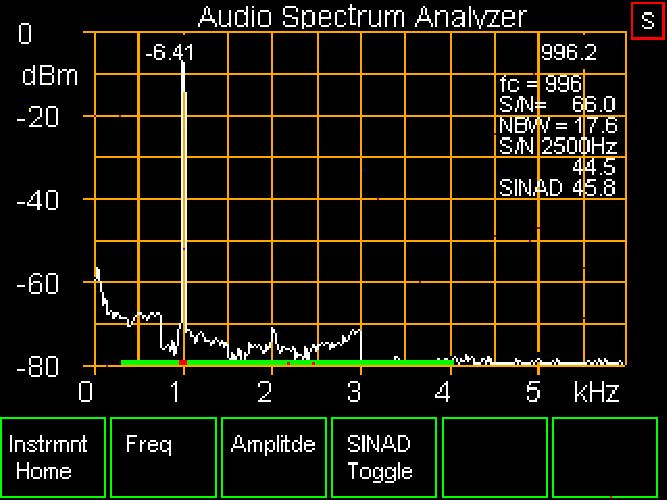
\includegraphics[scale=0.75]{./images/AVNA_020.pdf}
\caption{Spectrum Analyzer screen including SINAD measurements.}
\label{AVNA_020-label}
\end{center}
\end{figure}
%

SINAD is a measurement term that is used primarily to evaluate radio receiver performance.  Rather than trying to cover the definitions and uses of these terms here, please refer to the foot-noted references.\footnote{\textbf{\texttt{https://en.wikipedia.org/wiki/SINAD}}}\footnote{{\scriptsize\ \textbf{\texttt{https://www.electronics-notes.com/articles/radio/radio-receiver-sensitivity/what-is-sinad-signal-to-noise-and-distortion.php}}}}
%
For our ASA, the measurement bandwidth for noise is fixed at 300 to 4000 Hz.  The frequency center, as discussed above, is 996 Hz.  To allow for frequency errors in the signal generator for the 996 Hz tone (this may be an external generator that is part of an RF signal generator), the signal measurement adds 3 FFT bin powers together which is equivalent to a simple band-pass filter of about 40 Hz width, centered on 996 Hz.  The noise plus distortion power measurement excludes 5 bins, or about 60 Hz centered at 994 Hz.

With no signal present, the SINAD should show very close to 0.0 dB.  With increasing signal the SINAD will increase, representing the reduced competition of noise.

The other measurements shown are "\textsf{S/N}" which is the ratio, in dB, of the power in the signal bins to that in the sum of the two noise bands, scaled back to a single bin bandwidth.   The "\textsf{NBW}"  line is for the calculated Noise Band Width in Hz and refers to the noise in a single FFT bin (including windowing effects).   The "\textsf{S/N 2500}" is the same as "\textsf{S/N}" except 21.5 dB lower to reflect the wide band.  The reason for posting this tightly coupled number is the popular WSJT series of programs\footnote{\textbf{\texttt{https://physics.princeton.edu/pulsar/k1jt}}}that use this wide band S/N extensively.

\subsection{Discussion}
\label{subsect:ASADiscus}
Multiple FFT are averaged together to produce the ASA graph.  The width of the display can be varied in 2:1 steps from 3 to 48 kHz with the resolution bandwidth varying proportionally.  The normal scale is 80 dB which is 10 dB/div, but a 5 dB/div option is available along with offsets in 5 dB steps.  The peak level on the screen is indicated at the top left and the frequency of this peak is at the top right.  The level may be higher than the graphics peak as it is the sum power of the peak "bin" and the two adjacent ones.  The frequency indication includes interpolation between bins and has counter accuracy for stronger sine waves.  The input goes into the \q{T} Transmission port.  The calibration is in dBm into 50 Ohms and assumes that the 50 Ohm input terminator is switched in.

\section{Audio Signal Generators (ASG)}
\label{sect:ASG}
Included with the "Audio Test Instrument" firmware expansion were three signal generators and a fourth Gaussian White Noise generator. These four signals are summed, if turned on, and appear at the \q{Z} terminals.  These are for general use, but are not available when impedance or transmission measurements are being made.  The Signal Generators can produce sine waves or square waves all under direct control of the touch screen.  In addition, under USB serial control this capability  expanded to other waveform types, such as triangles (described in Section \ref{subsect:SerDes}).

Frequencies can be set from 10 to 40,000 Hz in 1 Hz steps, on-screen.  The amplitude is specified by the peak-to-peak value in volts.  The output impedance is 50-Ohms
%
\footnote{50-Ohms applies to the Z terminals.  A low impedance output of perhaps 1 Ohm is available at the BNC connector.  Either output can be used used.  }
%
 and the voltage displayed is that delivered to a 50-Ohm load. When open-circuited, the voltage will be double the displayed value.  For convenience, there is provision to turn each generator on and off while leaving the settings alone.

% \subsection{Description}
%MOVE/DELETE   >>>>>>>>>>>>>>>>>>>>>>>>>> 
%A couple of minor corrections.  In the example, the comments on the SigGen settings have the wrong amplitude levels.   The commands are OK.  The correct comments are \\ \\
 %\texttt{SIGGEN 1 1 1234.56 0.1 3}  // SG \#1 as a triangle wave 0.1 v p-p \\
 %\texttt{SIGGEN 4 1 0.0 0.003 0}  // SG \#4 Gaussian White Noise, $\sigma = 0.003$\\

\subsection{Instructions}
\label{subsect:ASGInstr}
As usual, we start with the Home screen of Figure  \ref{AVNA_000-label}.    Tapping on the button, "\textsf{Signal Gens}" brings up a Signal Generator summary screen such as seen here in Figure \ref{AVNA_021-label}.  This shows the frequency, voltage setting, on/off status and waveform for the three signal generators.  A fourth line is for the Gaussian White Noise generator and the nominal bandwidth for this is not adjustable.  When a generator is off, the on/off status appears in the pinkish color.  The control function of this screen is to allow bringing up one of four control screens for the individual generators.  We continue this by tapping on the "\textsf{SigGen 1}" button on the bottom row.
%
\begin{figure}[H]
\begin{center}
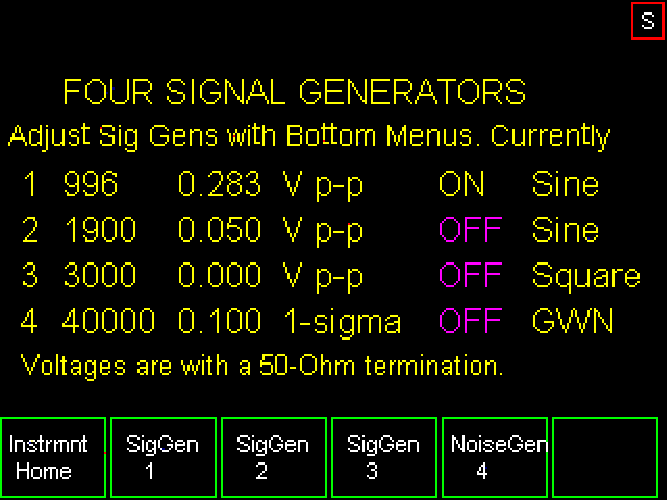
\includegraphics[scale=0.75]{./images/AVNA_021.pdf}
\caption{Signal Generator summary screen. }
\label{AVNA_021-label}
\end{center}
\end{figure}
%
This brings up Signal Generator \#1 control screen as seen in Figure  \ref{AVNA_022-label} below.
%
\begin{figure}[H]
\begin{center}
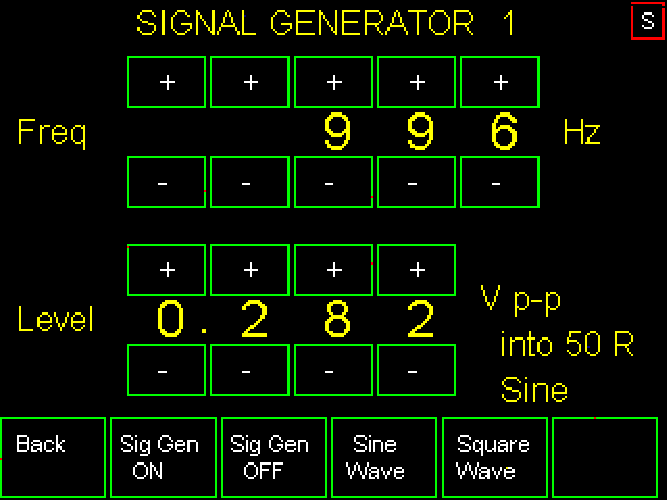
\includegraphics[scale=0.75]{./images/AVNA_022.pdf}
\caption{Signal Generator \#1 control screen  showing a 996 Hz sine wave at 0.282 Volts, p-p.  }
\label{AVNA_022-label}
\end{center}
\end{figure}
%
Here we see plus and minus buttons to control the individual digits for both frequency and amplitude.  In addition, we can turn this generator on and off with the "\textsf{SigGen ON}" and "\textsf{SigGen OFF}" buttons.  To the right of those buttons are a pair for selection of waveform, "\textsf{Sine Wave}" or "\textsf{Square Wave}".  You can make any of those changes now and then use the "\textsf{Back}" button to return us to the Signal Generator summary screen, Figure \ref{AVNA_021-label}.

Assuming that you have returned to the summary screen, you can tap on the "\textsf{NoisGen 4}" button to bring up that control screen, Figure  \ref{AVNA_024-label}.
\begin{figure}[H]
\begin{center}
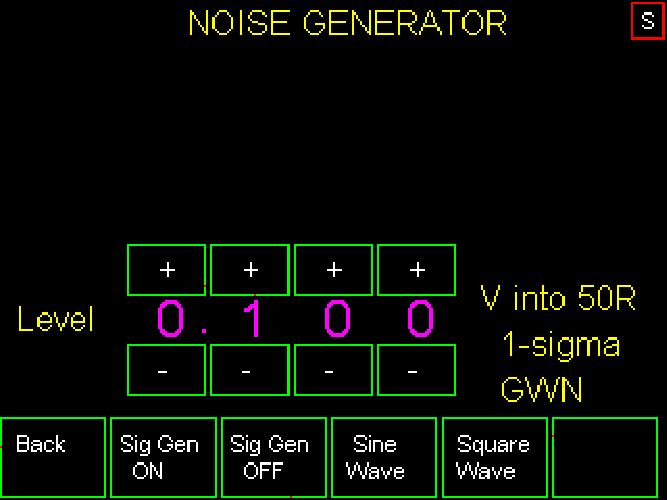
\includegraphics[scale=0.75]{./images/AVNA_024.pdf}
\caption{Gaussian White Noise generator with the 1-sigma value (standard deviation) set to 0.100 Volts when running into a 50-Ohm load.  The pinkish color of the 1-sigma value indicates that the noise generator is currently turned off.  The 1-sigma level is also the RMS value.}
\label{AVNA_024-label}
\end{center}
\end{figure}
%
This Noise Generator control is basically the same as the Signal Generators, except that there is no frequency control.  The spectrum of the noise is always flat, almost up to half the sample frequency, as set by the Spectrum Analyzer.  This is discussed further below.

\subsubsection{Signal Generator Waveforms}
\label{subsect:ASGWaveforms}
For sine waves, the waveform is excellent up to about 5/12th of the sample frequency, above which the amplitude drops off.   That corresponds to 40 kHz for the highest 96 kHz sample frequency.  For non-sine waves like our square wave, harmonics of the fundamental frequency are needed to build the waveform.  The missing high frequency pieces due to our limited band, cause the waveform to be distorted.  For waveforms like the square wave, this can be an important limitation and suggests keeping the generator frequency far below half the sample frequency, if possible. \footnote{For a more thorough treatment of the construction of a square waveform a sine wave and odd harmonics, see  \linebreak \textbf{\texttt{https://mathworld.wolfram.com/FourierSeriesSquareWave.html}}. \linebreak  The graph shows the result of limiting the spectrum to the fundamental, fundamental plus third harmonic, and fundamental plus third and  fifth harmonics.  The result gets closer with more harmonics, but the process requires many harmonics to not have obvious distortion. }
%
 In general, it pays to look at the waveform on an oscilloscope if the details are important.

If three sine waves are turned on at once, there can be times when all three will add together for a maximum voltage.  The sum of the three voltage settings should, therefore, be kept below the overload point of about 0.6 volts.

Note that all the control of the Signal Generators is also available from the Serial control using the USB plug.  Also note that over the Serial path the frequency can be controlled to the miliHertz, amplitude to the microVolt, and the waveform selections which also include triangle and two sawtooth waveforms.

\subsubsection{Noise}
\label{subsect:ASGNoise}
Signal  Generator \#4 produces Gaussian White noise.  There is an amplitude setting that corresponds to the 1-sigma voltage.  This is a convenient descriptor since the noise power is this voltage squared and divided by 50.  Being "White" noise, the power is spread uniformly across the band  of 0 to half the sampling frequency.  This means that the noise power density is the total noise power divided by half the sampling frequency,  expressed in Watts per Hz.  Keep in mind that the sampling frequency can be changed by the Spectrum Analyzer. For instance, if the 1-sigma noise level is 0.1 Volts, the power delivered to a 50-Ohm load is $0.1^2/50 = 0.0002$ Watts (0.2 milliWatts).   If the sample rate is 12 kHz the power is spread across 6 kHz so the power density is 0.2/6000 = 0.0000333 mW/Hz.  In dBm terms, this is -44.8 dBm/Hz.  As seen on the spectrum analyzer, with a noise bandwidth (for this sample rate) of 17.6 Hz, this will show about 17.6 * 0.0000333 = 0.000587 milliWatts per bin, or in dBm terms -32.3 dBm per bin.   This type of arithmetic allows setting the noise generator and the signal generators for any desired situation.

Looking at the noise waveform in the time domain,  the Gaussian statistics show that the 1-sigma value (standard deviation) is exceeded 68 percent of the time.  This is the common \q{bell} curve.  Note that for this Gaussian statistical distribution, the 1-sigma value as shown on the screen is also the RMS value. 

An interesting issue with this noise generator is to find the voltage setting that prevents overload, since Gaussian noise theoretically has no amplitude limit and the generator used here can achieve 12 times the 1-sigma voltage.  If you are looking for a high level of noise output, it is reasonable to set the 1-sigma point at 0.1 Volts overload (5-sigma = 0.50 Volts). For a 96 kHz sample rate, this will overload about every 20 seconds, on the average.  This will not be important for most experiments.

\textbf{Noise Bandwidth - }The term \q{White Noise} refers to the the spectral power being flat across all frequencies.   This sounds great, but of course, there is going to be an upper frequency limit.  The most obvious limit is half of the sampling frequency, the Nyquist limit.  In addition, the output DAC needs to reduce this range to prevent spurious alias outputs.  This limits our noise to about 5/6 of the half-sample frequency, or at the widest, about 5/6*48 kHz or 40 kHz.  Above this, the power spectrum drops off.  To indicate this restriction, the signal generator summary screen lists the noise by this restricted range.

\section{Noise Measurement}
xxx
\subsection{Description}
xxx
\subsection{Instructions}
xxx
\subsection{Discussion}
xxx

\section{Delay}
xxx
\subsection{Description}
xxx
\subsection{Instructions}
xxx
\subsection{Discussion}
xxx

\section{Screen Saving}
Screen saves are available for any AVNA1 screen (there are 21 different ones now), except the touch-screen calibration.   This can be especially useful for graphical displays, like the Spectrum Analyzer, but can also be a time saver for grabbing any screen.  All of the screen pictures in this manual were obtained with this function.  The screen saves can be stored in the $\mu$SD card on the Teensy 3.6, or if that is not convenient, the screen save can be transferred  to a PC  via the USB-Serial link.  All screen saves are in BMP format.

\subsection{Instructions}
\textbf{Screen Saves under touch-screen control - } To get started,  be sure to power up the AVNA1 with  an $\mu$SD card in the holder on the Teensy 3.6.  It is not necessary to have a serial terminal, like the Arduino Serial Monitor, connected.  But if you do, and the Monitor is open, it will display a \q{ls} / \q{dir} type of directory for the files on the $\mu$SD.  This will show all files on the card.   Be aware that the dates are all set for 1980 as the AVNA1 does not have a real-time clock.

In the upper-right hand corner of the screen is a small touch button with green outline and an "S".  This only appears if there is a $\mu$SD card in place.  Taking a screen shot only requires tapping on that button.  The outline will turn red during the several second screen-save period.  A file will be created with a unique name of 
the form \texttt{AVNA\_nnn.BMP} where \texttt{nnn} is a unique number in the range of 000 to 999.  These files are all at the root directory level of the card.  Any other files or directories on the card are ignored.  More screen save files can be created, as needed.

At this point there is no method for taking the saved BMP files other than to physically remove the $\mu$SD card.  Various adapters are available to read the  $\mu$SD card indifferent sorts of computers.

\textbf{Screen Saves under USB-Serial control - } There is capability to save a screen shot by a Serial Command.  The BMP save can be to an uSD card put into the Teensy 3.6 board, or it can be sent to the controlling PC as an Intel Hex file.  The Intel Hex is necessary as the USB-Serial connection cannot transfer full 8-bit bytes due to control code conflicts.  The Intel Hex format is somewhat clumsy for this job, but it works.  

Serial commands are all covered in Section 12.  The command follows, but refer to Section 12 for details, including the several file types and conversions of those file types.

\texttt{SCREENSAVE n} performs a single screen save of whatever is shown on the screen.  The parameter n is
\begin{description}
\item[n is 1] Send the screen BMP image over the USB Serial link using Intel Hex
\item[n is 2] Save the BMP image to the $\mu$SD card, exactly as is done with the touch screen command.
\end{description}

\section{AVNA1 Calibration}
\label{sect:Cal}

Calibration allows us to adjust our measurements to be in some agreement with various standards.  This gives us control over, say, the voltage difference between our Volt, and the "standard Volt."  Since  most of us don't have direct access to the standard Volt
 \footnote{Although not important to our measurements, the standard Volt is an amazing collection of strange hardware
\textbf{  \texttt{https://en.wikipedia.org/wiki/Josephson\_voltage\_standard}  }
}
we instead find ourselves at the end of a succession of measurement transfers, using perhaps a commercial digital Voltmeter as our local comparison device.  In the big picture, calibration is complex and sometimes esoteric, but at the home lab level, we just use the best reference(s) we can find! 

So, in that context, the calibrations needed for the AVNA1, including the Audio Test Instrument additions are as follows.

\begin{itemize}
  \item AVNA Impedance calibration is a combination of internal resistor values and measurements made of the stray capacity and resistance by means of the Setup Commands, described in Section \ref{subsect:SerSetup}.
  \item AVNA Transmission calibration performed as part of the measurements of Section \ref{subsect:SerCmd}).
  \item AC Output Voltage calibration performed using an external voltmeter, described below.
  \item AC Input Vector Voltmeter and Spectrum Analyzer calibration performed using the previous Output calibration.
  \item Touch Screen Calibration that aligns the touch screen with the visual screen, also described below.
\end{itemize}

\subsection{Instructions}
\label{subsect:CalInstr}
\subsection{Touch Screen Calibration} There is some variability to the scaling of the touch screen.  Calibration ties the grid for the visual screen to that of the touch screen, that operates independently.  The original AVNA1 software used nominal x and y calibration values.  With the addition of this Touch Screen Calibration,   tapping at the upper-left corner and the lower right corner, allows us to find the lowest and highest x and y touch values.

Let's go through this step-by-step.  Starting at the usual home screen, we tap on "\textsf{Service \& Cal}" button. This brings up the screen for selecting various calibrations.  We tap on "\textsf{Touch Cal}" to bring up a screen with a list of the needed steps. Note that once a touch screen calibration is started, it should be completed.  Follow  the three steps on the screen, observing the minimum and maximum values that have been found.  Any number of taps is allowed.  Finally,  the upper-right corner is tapped at which point the values are made permanent. 

Multiple taps with a stylus may find slightly more extreme values improving the calibration.   In using this, be sure to tap on the screen many times, seeing if more extreme values can be found.  Also, there is no true "Cancel" for this test, except that if the upper-right corner is tapped before any  other, it will continue to use the old values.  It is safe to just re-calibrate the screen.  The test is fast and can be redone any number of times. 

After tapping on the upper-right corner, a confirmation screen is displayed, showing that the new values have been registered.  If no corner tapping was done, this last screen just shows the current stored calibration values.

\subsection{Voltage Input Calibration} We need a basic reference to correct for variations in the gain of analog circuitry.  The preset values should be close, but variations are inevitable.  This calibration uses an external generator of known amplitude of sine wave set to 0.100 Volts RMS which is the same as 0.2828 Volts peak-to-peak. The frequency is not critical, but should be in the 1000 Hz range.  Apply this to the \q{T} terminals.  The 50-Ohm termination can be on or off as the important item is the voltage at the terminals.  Some signal sources provide calibrated output voltages.  This may be your best calibration standard.  Every bit as good is to measure this voltage carefully with an AC Voltmeter.  Again, the Voltmeter measurement should be done with the generator connected to the \q{T} input terminals.

If we do this calibration step-by-step, after connecting our 1000 Hz signal source,  we start with the Home screen and tap on "\textsf{Service \& Cal}" button. This brings up the screen for selecting various calibrations.  We tap on "\textsf{V Input Cal}" to bring up the measurement screen, including instructions for this calibration.  Tap on "\textsf{Measure}" and wait for the measurement to complete.  Assuming that the answers are reasonable, tap "\textsf{Done}" to go back to the Calibration Home screen.  This calibrates the voltage amplitude for ASA and VVM use.  The AVNA uses only relative voltages and does not need this type of calibration.

As an alternative to the external calibrated generator,  we can use the internal Signal Generator \#1 (SG\#1) and an external Voltmeter.  The problem with this is that the generator is not calibrated at this point in time and needs to be brought to the needed 0.100 Volts RMS by trial-and-measurement.  Instructions for setting SG\#1 are in Section 6.  The frequency should, of course, be set to 1000 Hz, and SG\#1 must be enabled.   This method relies completely on the voltage measured with a good external voltmeter.

\subsection{Voltage Output Calibration} Now we need to calibrate the Audio Signal Generator (ASG) output levels.  This function assumes that the Voltage Input Calibration is correct and adjusts the ASG levels to correspond.  Therefore, this calibration \textit{must} always follow a successful Voltage Input Calibration.  For this to work, the non-ground, hot \q{Z} and \q{T} terminals need to be wired  or test-clipped together.  Then follow the on-screen instructions.  This is very close to the same step-by-step procedure followed for the Voltage Input Calibration. 


\section{System Issues}
\label{sect:Sys}

\textbf{SIMULTANEITY} - We have limited input and output ports.  Combinations of Instruments and functions is limited by this.  Usually, this will be caught by the firmware if you try the impossible.  For instance, the four signal generators are turned off when the Vector Network Analyzer is running.  What we can do is to have multiple generators on at once.  For instance, the use of two (or three) generators for inter-modulation analysis is works well up to the overload point.  This, in part, is because the analog output amplifier uses much negative feedback and is quite linear.  Likewise combining signals and noise works well for setting specific S/N ratios, or other experiments.

\textbf{COHERENCY} - If multiple waves are added together, and they are at non-harmonic related frequencies, the relative levels change at a fast rate.  In the other extreme, if the two
waves are at the same frequency, they maintain a constant phase relationship. This can alter measurement results, depending on the phase. As implemented here, the phase relationship between two generators is a random  value.  For these reasons, you should not measure inter-modulation distortion with frequencies, such as 1000 and 2000 Hz.  Standard frequency pairs, such as 700 and 1900 Hz or 60 Hz and 7000 Hz support predictable results.

\textbf{EEPROM Update} - We keep adding items to the permanent EEPROM memory in the Teensy (this is Flash memory set up to emulate EEPROM).  At startup, the program checks the version that was used to write the EEPROM and adds nominal values for anything that was added after that version.  This prevents overwriting tune up values or the like.  If everything is up-to-date, the Serial monitor, at startup, should say, "Loading EEPROM data; Turn-on EEPROM version was 80; EEPROM Load of 536 bytes."  The first time version 80 is run, there will be notes about the updating of the data.

\section{AVNA Serial Interface}
\label{sect:Ser}   % Added labels Jan2020 RSL
% xxx

\subsection{Description}
\label{subsect:SerDes}
Commands are entered by the USB serial link to the Teensy 3.6 board. The Teensy appears to the Host computer as a \q{Serial Device}. As such, it can be controlled by an external program for graphing and the like.  For manual control, the \q{Arduino Serial Monitor} that is accessed from the Arduino IDE under the menu \q{Tools}Äù is useful.  This monitor (terminal) supports CTRL-C copy and data can be gathered that way.

\subsection{General Command Syntax}
\label{subsect:SerSyn}
The format for all commands going to the AVNA is
\begin{verbatim}
    CMD param1 param2 ....
\end{verbatim}
where \texttt{CMD} is 1 or more characters, and the number of parameters varies.  Only capital letters are valid for the \texttt{CMD} field. Error checking is not done on parameters.  If 5 parameters are allowed, and only the first two are to be set, the last 3 do not need to be sent.  Also the delimiter is shown as a space, but commas can be used as well.

For common commands used for manual entry, there are single character short cuts.  For instance, \texttt{FREQ} and \texttt{F} are equivalent. See Section 5 for a complete list.

\subsection{Operational Commands}
\label{subsect:SerCmd}
\begin{description}

\item[\texttt{ZMEAS refR}]
This command sets the measurement to Impedance and the reference resistor value to \texttt{refR}.  Valid \texttt{refR} values are either 50 or 5000 ohms.

\item[\texttt{TRANSMISSION refR}]
This command sets the measurement to Transmission and the reference resistor value to \texttt{refR}.  Valid \texttt{refR} values are either 50 or 5000 ohms.

\item[\texttt{FREQ} \texttt{f}]
This command sets the measurements to a single (non-sweep) frequency. The frequency is set to \texttt{f} which can be either an integer or a decimal number from 10 to 40000.   The parameter \texttt{f} regards 100.0 and 100 as the same.  The achieved frequency may be slightly different than \texttt{f} to provide proper averaging of the multiplier outputs.

\item[\texttt{SWEEP}]   No parameters are used.  The 13 frequency sweep is set up, but not run (see \texttt{RUN} command).

\item[\texttt{LINLOG rs ts}]  changes the units used for outputs to the serial monitor,
  or to the Touch Display.  The four numbers following the \texttt{LINLOG} command set:
\begin{description}
\item[\texttt{rs} = 0]  Reflection coefficient to Serial in dB, and phase in degrees
\item[\texttt{rs} = 1]  Reflection coefficient to Serial in magnitude (0,1) and phase in degrees
\item[\texttt{rs} = 2]  Reflection data to Serial as equivalent Series Impedance or Parallel Suseptance (see \texttt{SERPAR} command)
\item[\texttt{ts} = 0]  Transmission data to Serial in dB, and phase in degrees
\item[\texttt{ts} = 1]  Transmission data to Serial in magnitude and phase in degrees
\end{description}
   Default is the original values, for backward compatibility:\mbox{ \texttt{LINLOG 2 1}.}

   Short commands work if you do not want to change the touch display. For instance, \texttt{LINLOG 0} will
   just make the serial output in dB and degrees for impedance.

   The command \texttt{LINLOG} without any parameters will return the current settings, such as \texttt{LINLOG 0 0}.

   Settings are saved in EEPROM and so survive the power shutdown.

   This makes a variety of Serial outputs available.  For instance, for impedance measurement of a 200 uH inductor at
   10 KHz.:

    With \texttt{LINLOG 0 0}:  the serial monitor shows a series of lines:
      \\ \texttt{10000.000 Hz\\ Return Loss = 0.486 dB\\  Phase = 150.74}

    With \texttt{LINLOG 1 0}:  the serial monitor shows a series of lines:
      \\ \texttt{10000.000 Hz\\ Reflection Coefficient = 0.94565\\  Phase = 150.74}

    With \texttt{LINLOG 2 0}:  the serial monitor shows a series of lines:
      \\ \texttt{10000.000 Hz\\ Series RX: R=1.494 X=13.042 L= 207.6uH Q=8.73}
      \\ \texttt{10000.000 Hz\\ Parallel GB: G=0.008667760 B=-0.075683906 R= 115.37 L= 207.6uH Q=8.73}

    With \texttt{LINLOG 2 0} and \texttt{SERPAR 1 0} the serial monitor omits the suseptance:
      \\ \texttt{10000.000 Hz Series RX: R=1.494 X=13.042 L= 207.6uH Q=8.73}

    If the output is intended to be read by a program, you do not want all the annotation.  When this is stopped by
    \texttt{ANNOTATE 0}, the data fields become comma separated, which spread sheets are happy with.  For instance, the inductor
    measurement with "\texttt{LINLOG 1 0} looks like
      \texttt{10000.000,0.94565,150.74}.
    The second number controls the transmission format in a similar manner, but options are only 0 or 1.

\item[\texttt{CAL}]
No parameters are required.  This is an immediate calibrate of either Z or T measurements at either a single frequency or all 13 sweep frequencies.  This must follow \texttt{FREQ} or \texttt{SWEEP} and \texttt{ZMEAS} or \texttt{TRANSMISSION} to do the proper calibrate.  This command must precede \texttt{RUN}.  Note that component connections can be left in place for \texttt{CAL} of impedance measurements, but transmission measurements need a reference path for proper calibration.

\item[\texttt{RUN nRun}]
This command causes the selected measurement to occur, either single frequency or a full set of swept measurements.  The parameter, \texttt{nRun} is the number of measurement sets made.  An \texttt{nRun} value of 0 causes a continuous set of measurements to be made.  That is, \texttt{RUN 1} is a single measurement set;  \texttt{RUN 27} does 27 sets and stops.  Any new command will break the \texttt{RUN} command, so \texttt{RUN 0} is not really forever.

\item[\texttt{POWER}] No parameters are required.  This is a power sweep of transmission measurements at a single frequency.  Implementation is in place, although not thoroughly tested.  Documentation is coming.

\item[\texttt{SAVE}]   No parameters are required.  This saves the current state to \mbox{EEPROM} for the next power down.  This is seldom needed, as it is automatic if a parameter, such as the reference impedance is changed.

\item[\texttt{LOAD}]   No parameters are required.  Complements \texttt{SAVE} and retrieves settings from EEPROM.  Also seldom needed.

\item[\texttt{DELAY msDelay}]   sets a delay between repeated runs (see \texttt{RUN} command).  The parameter \texttt{msDelay} is the amount of delay in milliseconds.  This applies to measurements over the serial link and not the touch display.

\item[\texttt{CALDAT}]  Not used at this time.

\item[\texttt{SERPAR ser par}] sets type of output data sent back to a host PC, during Z measurements, where:
\begin{center}
\begin{tabular}{c l}
ser = 0 & Do not transmit series R-X data \\
ser = 1 & Transmit series R-X data \\
par = 0 & Do not transmit parallel G-B data \\
par = 1 & Transmit parallel G-B data \\
\end{tabular}
\end{center}

For instance, the command \texttt{SERPAR 0 1} would include data for parallel G-B representation of the measured impedance.

The normal representation for an impedance is the (\texttt{ser = 1}) series form specified by a resistance, R, and a reactance, X connected in series..

When \texttt{par = 1}, representation is the mathematically related parallel conductance, G, and susceptance, B.

Note that annotation of the general form "R=" can be added for both impedance forms by the "\texttt{ANNOTATE 1}" command.

Avoid having both \texttt{ser = 0} and \texttt{par = 0}, as there will be no output to the PC, and there will be no obvious reason.

Unless modified by a \texttt{SERPAR} command, the unit defaults to \newline \texttt{SERPAR 1 1}.

\item[\texttt{TEST rys sws}] This command sets the three relays and switches .  This is not normally used for measurements, as the proper relay settings will be made by a measurement command, such as \texttt{ZMEAS}.  (See TestCommand()  in the .INO)

\item[\texttt{BAUD}]   Do not use.  All USB communications on the USB port are at 12 MBits/sec

\item[\texttt{ANNOTATE 0} or \texttt{1}]  Responses can have annotation (1) or no annotation (0), over the serial communication.

\item[\texttt{VERBOSE 0} or \texttt{1}]  For (1), extra information is transmitted. For (0), no extra information is transmitted.

\item[\texttt{SCREENSAVE n}] does a single save of whatever is shown on the screen.  The parameter n is
\begin{description}
\item[n is 1] Send the screen BMP image over the USB Serial link using Intel Hex
\item[n is 2] Save the BMP image to the uSD card, exactly as is done with the touch screen command.
\end{description}

For example, "\texttt{SCREENSAVE 1} $<Enter>$" will cause the transmission of 14,409 lines of Intel Hex.

For n=2, there is serial feedback in the form of the new file name, only if you have set "\texttt{VERBOSE 1}".  Otherwise it is silent.

Now for n=1, the next step is to create a file from the huge collection of hex data at the Serial Monitor.  After printing the hex data, the cursor will be at the bottom.  Starting at that point, the steps are:
\begin{enumerate}

\item Starting with the right end of the last line, highlight that line, "\texttt{:00000001FF}". Then, being careful to not click in the text area, use the scroll bar to go to the top of the hex text. Hold down the Shift key and carefully left-click on the start of the first, "\texttt{:020000040000FA}" line. The entire hex text should now be highlighted.

\item To get the hex to the clipboard, just hold down the CTRL key and hit '\texttt{c}'. There is no feedback from this. There is no menu item for this step, only the Ctrl-c.

\item Paste this entire hex area into your text editor and save it to a a file with type \texttt{.hex}. That might be (for Linux) \\ \texttt{/home/me/Documents/myscreen.hex}.  If you are not using Linux, the file directory format will be different, but the file names can be the same.
\end{enumerate}

To this point the procedure is very similar for different operating systems.  The next step is to convert the HEX file to a BMP file and that varies depending on operating system.   What follows is for Linux and Windows 10.  textit{Does anyone have a procedure for Mac OSX?}  


\textbf{HEX to BMP file conversion on Linux}:
\begin{enumerate}
\item Determine if your computer has \texttt{objcopy} installed by typing \texttt{objcopy -version} in a terminal.  If it is not present, download it with your apt-get procedure.

\item Open a Terminal and navigate to the directory location of the HEX file, such as \texttt{cd /home/me/Documents}.  Now we will create the \texttt{.bmp} bitmap file, \texttt{myscreen.bmp}, that was the goal.  Using the nifty \texttt{objcopy} utility, the command is \texttt{objcopy -I ihex -O binary myscreen.hex myscreen.bmp}.

\item The HEX file can be deleted, if desired.
\end{enumerate}

\textbf{HEX to BMP file conversion on Windows 10}  Thanks to Ray, W7GLF, for working this out:
\begin{enumerate}
 \item Download the latest version of the application of srecord from sourceforge:
\linebreak
\textbf{\texttt{https://sourceforge.net/projects/srecord/files/srecord-win32/}}
\linebreak

The file name will be similar to \texttt{srecord-1.64-win32.zip}.  Copy the zip file into a folder of your choice.  Right click on the file in file explorer and select \texttt{Extract All}.  Leave the folder to extract to as is.  When the extraction is done you will have a number of files in the subfolder.  The one we care about is named \texttt{srec\_cat.exe}.  You can copy this file wherever you like.  You can delete the other files if you wish or read the pdf to see other record features.

\item Start a command window to run the program.  To start a command, right click the Start Button icon in the lower right edge of the screen.  Select the run menu and type \texttt{cmd.exe <return>}.  You will then need to go to the folder where you put texttt{srec\_cat} using the cd (change directory) command. 

Type \begin{verbatim} cd /d c:\myVNA\srecord\end{verbatim} if you put the srec\_cat.exe file in that folder.

Alternatively you can use file explorer and navigate to the folder that contains the file \texttt{srec\_cat.exe}.  Hold the CTRL KEY and the Shift KEY at the same time and right click on the surrounding folder.  A menu will appear and one of the choices should be Open PowerShell Menu Here.  Click on that and a PowerShell window should appear.  It will already be in the correct directory.  You still need to start a normal command window here so type \texttt{cmd.exe <return>} to start the command window from within the powershell window.  

\item You can convert the Intel hex file by typing the following command in the command window:  \texttt{srec\_cat  <input file name> -intel --address-length=4 -o <output file name>  -bin}.

For example if your input file is AVNAScreen.hex you could type: \texttt{srec\_cat  AVNAScreen.hex -intel --address-length=4 -o AVNAScreen.bmp –bin}.
\end{enumerate}
\end{description}

If you are using HEX to BMP conversion programs other than shown above, be aware that the \texttt{.hex} file has three hex encoded bytes per pixel. There are 320 x 240 pixels, or a total of 230,400 bytes of data. This is more bytes than a 16-bit address can handle. Intel Hex originally was 16-bit only, but later extended to 32-bits with the "type 4 extended address." Most  Intel Hex readers conversion programs handle this extended addresses, but some do not.

Also, any graphics program will recognize the BMP file type. However, it still maybe desirable to lossless compress the file to, for instance, a \texttt{.gif} file. The redundancy in the screens \texttt{.bmp} is very high and the savings from compression are quite useful but not required.

\subsection{Setup Commands}
\label{subsect:SerSetup}
\begin{description}

\item[\texttt{PARAM1 num refR50 refR5K}]
This command is used to set the "exact" values of the two reference resistors (\texttt{refR50} and \texttt{refR5K}), if known.  \texttt{refR50} and \texttt{refR5K} default to the design values of 50.00 ohms and 5000.00 ohms respectively. The parameter \texttt{num} is either 0 or 99. A value 0 causes the reference resistor values to be set to the two parameter values, \texttt{refR50} and \texttt{refR5000}.  A num value 99 causes \underline{ALL} EEPROM values to be set to the defaults, including \texttt{PARAM2} below. \textit{Use the 99 value with care.}  An example is \q{\texttt{PARAM1 0 50.22 5017.3}} which sets the two reference values, \texttt{refR50} and \texttt{refR5K}, to 50.22 and 5017.3 ohms respectively.  \texttt{PARAM1} with no following parameters returns the current two reference resistor values.

\item[\texttt{PARAM2 capInput resInput capCouple seriesR seriesL}]
Serves the changing of correction factors for the impedance measurements.
 For instance,
 \begin{verbatim}
 "PARAM2 37.0  1000000.0    0.22    0.07   20.0"
 [units]  pF      Ohm        uF      Ohm    nH
 \end{verbatim}
 sets the input shunt capacity, the shunt resistance, the coupling cap, lead resistance and lead inductance.
Note \texttt{capInput} is the most likely item to change, and it can be changed with simply "\texttt{PARAM2 34.8}"
To obtain current values, type  \texttt{PARAM2}  with no parameters

\item[\texttt{TUNEUP n}] is a set of six commands (\texttt{n = 1, 2, 3, 4, 5, or 6}) used at setup time or whenever values need to be checked. These are the values that correct for circuit \q{stray} components to improve the accuracy of impedance measurements. This command is available only over the serial port (no touch screen). It is directed manually, since components, opens, and shorts need to be connected.  These measurements determine the six values that are listed by the two commands, \texttt{PARAM1} and \texttt{PARAM2} (not including the non-critical 0.22 uF coupling capacitor).  The intention is that \texttt{TUNEUP} be used in 1 to 5 order. (See the separate write-up on doing the tuneup.) The \texttt{TUNEUP} family includes:
\begin{description}
\item[\texttt{TUNEUP}] with no "\texttt{n}" prints a summary of this procedure.

\item[\texttt{TUNEUP 1}]  with a short circuit on the Z terminals measures the stray resistance and inductance (\texttt{seriesR \& seriesL}).

\item[\texttt{TUNEUP 2 REXT50}] (1) find a resistor around 50 ohms, (2) as accurately as possible, measure the actual resistance of this resistor (in ohms), (3) then run \texttt{TUNEUP 2 REXT50};  enter the actual measured value (which will probably not be exactly 50 ohms) in place of \texttt{REXT50}.

\item[\texttt{TUNEUP 3 REXT5K}] (1) find a resistor around 5000 ohms, (2) as accurately as possible, measure the actual resistance of this resistor (in ohms), (3) then run \texttt{TUNEUP 3 REXT5K};  entering the actual measured value (which will probably not be exactly 5000 ohms) in place of \texttt{REXT5K}.

\item[\texttt{TUNEUP 4}] with the Z terminals open measures the internal 1 Megohm resistor and the input capacity (\texttt{resInput \& capInput}).

\item[\texttt{TUNEUP 5}] causes the six values to be made permanent.

\item[\texttt{TUNEUP 6}] reverts to the original six values that were used before \texttt{TUNEUP} was started.
\end{description}
Any of the steps can be omitted, \eg  if no precise resistor around 50 ohms is available.  But, the ascending order from 1 to 5 is important, in that, for instance, the value of the 5000 ohm reference affects the open circuit answers.

\end{description}

\subsection{Example of Commands}
\label{subsect:SerEx}

As an example, a swept measurement of transmission data, as commanded for non-manual use, might look like the following:  This does 1 Hz steps from 950 to 1050 Hz.  Obviously, the \texttt{F xxx R 1} repetition would be done by a loop in a control program.
\newpage
\begin{verbatim}
T 50
SWEEP
CAL
(Connect device to be measured for transmission)
F 950
R 1
F 951
R 1
F 952
R 1
. . .
F 1049
R 1
F 1050
R 1
\end{verbatim}

\section{Shortened Form of Commands}
\label{subsect:SerShort}
\begin{center}
\begin{tabular}{|c||c|} \hline
\textbf{Full Command}   &  \textbf{Abbreviation}  \\ \hline \hline
\texttt{ZMEAS}    &   \texttt{Z} \\ \hline
\texttt{TRANSMISSION}   &   \texttt{T} \\ \hline
\texttt{FREQ}   &   \texttt{F} \\ \hline
\texttt{CAL}   &   \texttt{C} \\ \hline
\texttt{RUN}   &  \texttt{R} \\ \hline
\texttt{POWER}    &  \texttt{P}  \\ \hline
\texttt{SAVE }   &   \texttt{S}  \\ \hline
\texttt{LOAD}    &   \texttt{L}  \\ \hline
\texttt{DELAY}    &   \texttt{D}  \\ \hline
\texttt{CALDAT}   &    none \\ \hline
\texttt{SERPAR}   &   none   \\ \hline
\texttt{PARAM1}   &   none  \\ \hline
\texttt{PARAM2}   &   none  \\ \hline
\texttt{TUNEUP}   &   none  \\ \hline
\texttt{LINLOG}    &    none  \\ \hline
\texttt{BAUD}        &   \texttt{B}  \\ \hline
\texttt{ANNOTATE}   &   \texttt{A}  \\ \hline
\texttt{VERBOSE}     &   \texttt{V}  \\ \hline

\end{tabular}
\end{center}

\subsection{Discussion}
xxx


%\input{EW-AcroList.tex}
\end{document}
